% Alles was man wissen muss um das Konzept zu verstehen.

\chapter{Hintergrund}
\label{sec:hintergrund}

In diesem Kapitel werden die Grundlagen erläutert, welche nötig sind, um die Konzepte und Realisierung genauer zu verstehen. Unter anderem wird auf die Grundlagen des Networkings, die verschiedenen Arten des Hostings, Datenspeicherung und Transfer, Informationskontrolle sowie Interest Management, Matchmaking und Synchronisation eingegangen.

\section{Grundlagen des Networkings in Online-Videospielen}

Die Grundlagen des Networkings in Videospielen lassen sich in zwei große Bereiche kategorisieren. Die physische und die logische Plattform. 

Die physische Plattform setzt sich aus den physikalischen Komponenten zusammen, die vereint eine Infrastruktur bilden. Hierzu zählt Hardware, welche in Rechenzentren eingesetzt wird, das lokale Endgerät wie z. B. ein Smartphone oder Personal Computer. Ebenfalls zählen Kabelleitungen und drahtlose Übertragungswege dazu. 

Online-Videospiele sind aus technischer Sicht auch nichts anderes als Anwendungen, welche miteinander kommunizieren. Die physischen Restriktionen wie Bandweite und Latenz können also ebenfalls auf den Kontext der Multiplayer-Spiele angewendet werden. Die Menge an Informationen, welche über ein Netzwerk versendet werden, kann je nach Spieltyp sehr hoch skalieren, weshalb sich die Entwickler eines Multiplayer-Spiels intensiv mit der logischen Plattform beschäftigen müssen.

Die logische Plattform baut auf der physischen Plattform auf und nutzt ihre Ressourcen. Sie kann unterteilt werden in Kommunikation zwischen Clients und Server, Datenspeicherung und Transfer sowie Kontrolle des Spielflusses. Auf diese drei Punkte wird in den folgenden Sektionen näher eingegangen.

\cite{Smed.2002c}


\section{Verschiedene Arten des Hostings}
\label{arten_des_hostings}

Die Kommunikation zwischen Clients und Server kann in zwei verschiedenen Varianten vorkommen:

\textsf{\Large Client Host:}

\begin{figure}[H]
	\centering
	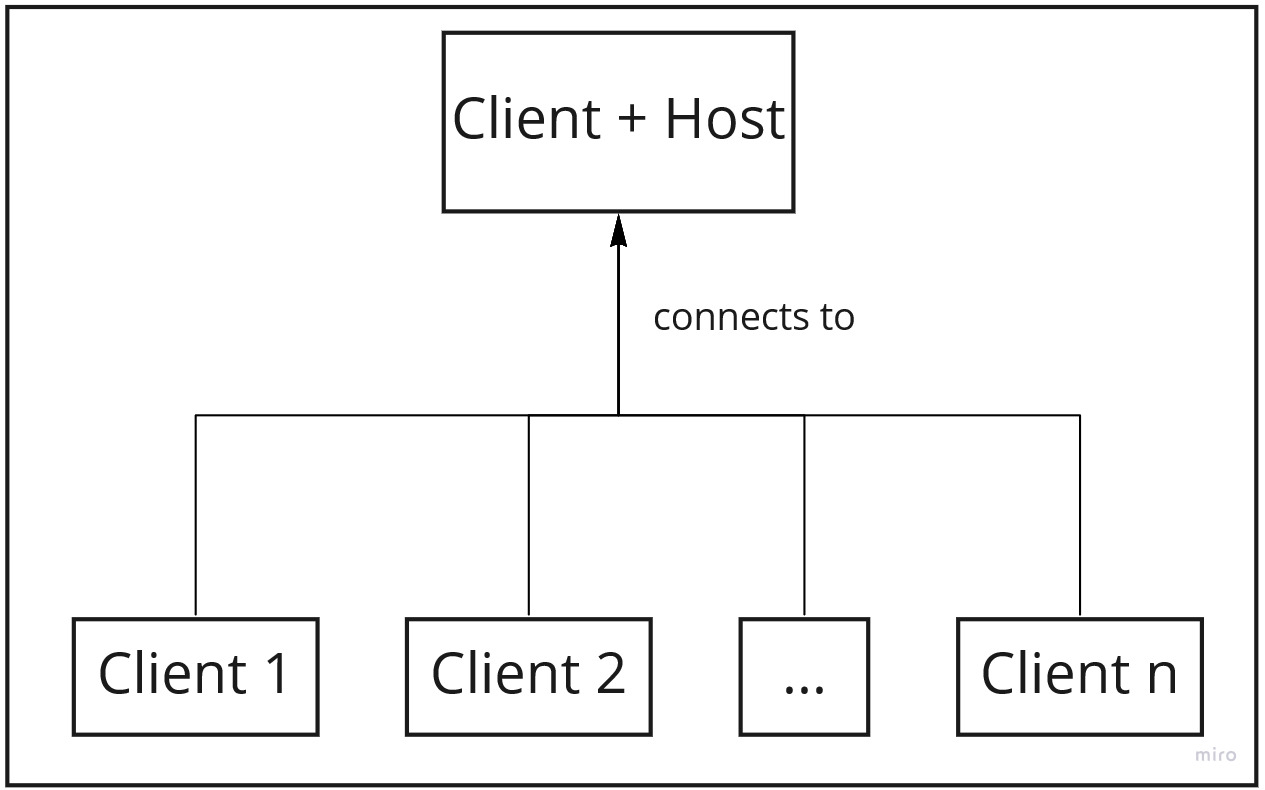
\includegraphics[width=150mm]{images/Client_Host.jpg}
	\caption[Client-Server Modell]{Das Client-Host-Modell einfach veranschaulicht}
	\label{pic:Client_Host}
\end{figure}

Bei dieser Variante wird der Serverprozess auf demselben Gerät ausgeführt, auf dem auch eine Client-Instanz gestartet wurde. Ein Spieler übernimmt also selbst das Hosting. Andere Clients haben die Information, welcher Client einen Serverprozess besitzt und wie sie sich dorthin verbinden können. 

\textbf{Vorteile:} Die Unabhängigkeit von Hardwareressourcen für Entwickler Dieses 'Problem' wird an die Spieler ausgelagert. 

\textbf{Nachteile:} Da der Serverprozess nun ebenfalls auf einem Gerät läuft, auf welches Spieler Zugriff haben, gibt es ebenfalls mehr Möglichkeiten des Hacking (Spielmanipulation) \cite{Wikipedia.2021h}. Die Entwickler haben keinerlei Einfluss auf die Serverprozesse, welche ein Spieler startet.
\cite{Smed.2002}

\newpage
\textsf{\Large Client Server:}

\begin{figure}[H]
\centering
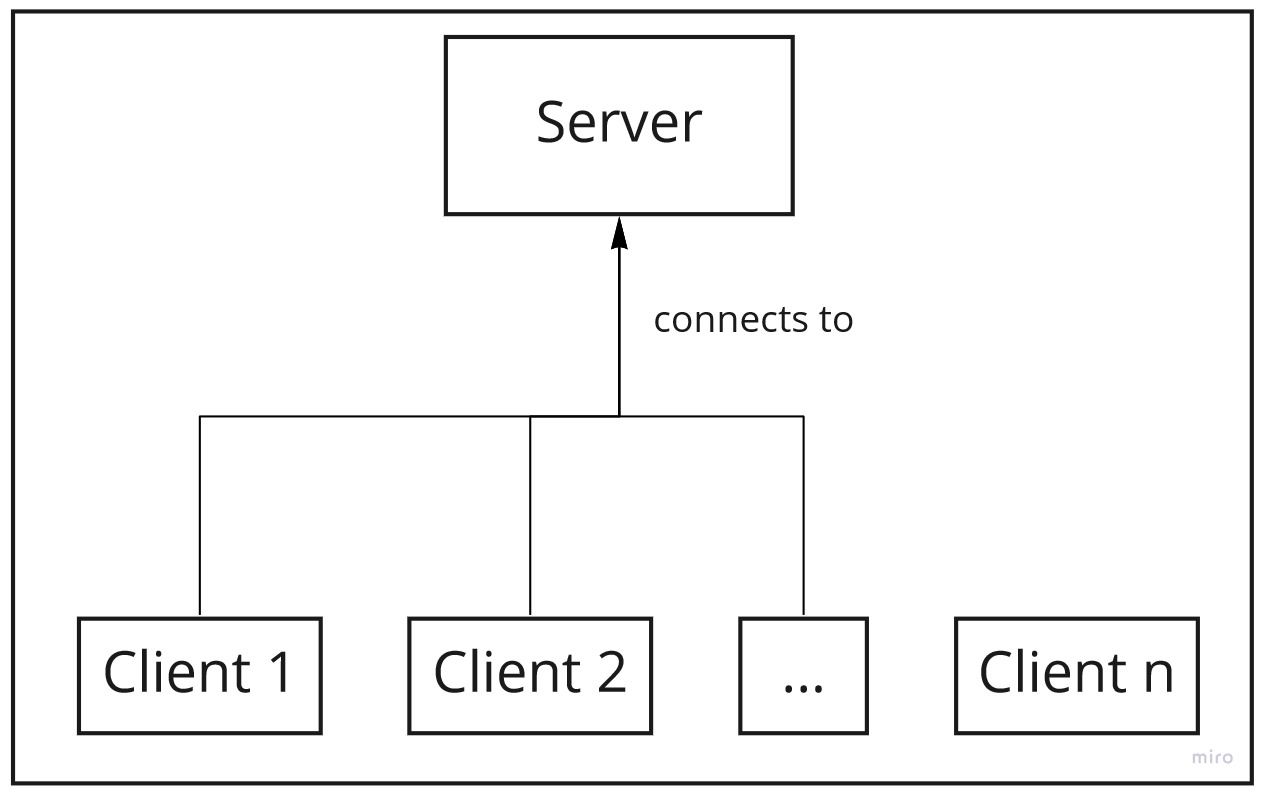
\includegraphics[width=150mm]{images/Client_Server.jpg}
\caption[Client-Server Modell]{Das Client-Server-Modell einfach veranschaulicht}
\label{pic:Client_Server}
\end{figure}



Diese Variante trennt Client und Server physikalisch voneinander. Serverprozesse werden außerhalb einer Client-Umgebung gestartet und verwaltet. Clients haben einen (oder mehrere) zentrale Zielsysteme, zu welchen sie sich verbinden können.

\textbf{Vorteile:}

Mehr Kontrolle auf Seiten der Entwickler, Hacking ist deutlich erschwert. Die Software-Architektur kann verhindern, dass spielentscheidende Daten nicht in der Hand der Spieler liegen, und somit ein sicheres und faires Spiel gewährleistet werden kann.
\cite{Smed.2002}

\textbf{Nachteile:}

Die Kosten für Hardware und Bandbreite skalieren mit den Spielerzahlen. Diese Tatsache könnte sehr schnell hohe Kosten verursachen. \cite{Deng.2018}

Bei einer simplen, monolithischen Architektur kann dieses Modell dazu führen, dass die Hardware, welche als Server fungiert zum 'Single Point of Failure' wird. Das bedeutet, dass ein Ausfall des zentralen Spielservers dazu führen kann, dass ein Großteil der Spielerfahrung nicht mehr spielbar ist.

\section{Datenspeicherung und Transfer}

Um das bestmögliche Spielerlebnis zu ermöglichen, sollte innerhalb der Entwicklung von Multiplayer-Spielen darauf geachtet werden, dass spielentscheidende Daten schnellstmöglich zwischen den Clients synchronisiert werden. Wie auch bei anderen Echtzeitsystemen \cite{Wikipedia.2021} kommt es also auch bei der Entwicklung von dieser Art von Software darauf an, Daten zu serialisieren (Konvertierung der Daten für die Übertragung über das Netzwerk) \cite{Wikipedia.2019}. 

Daten unterscheiden sich im Kontext der Online Spielentwicklung grundsätzlich nicht großartig von anderer Software. Typischerweise werden Programmiersprachen wie C\# oder C++ genutzt, um Klassen und Datenstrukturen zu erstellen, welche die eigene Spiellogik abbilden. \cite{Glinka.2008}

Das folgende Klassendiagramm zeigt zwei simple Klassen. Eine Klasse, welche den Spieler abbildet sowie eine Klasse, welche alle Spieler verwaltet.

\begin{figure}[H]
	\centering
	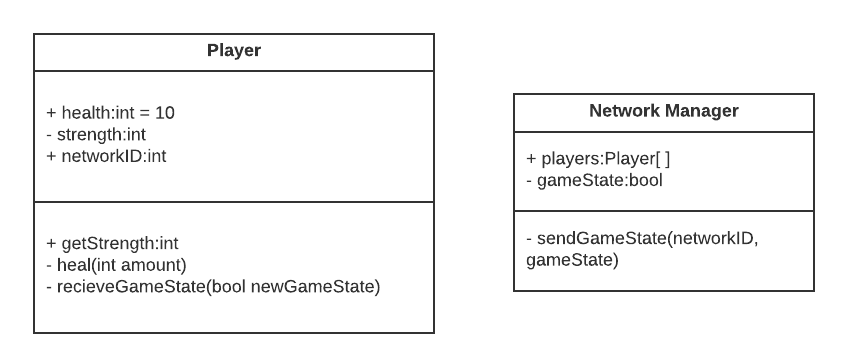
\includegraphics[width=150mm]{images/UML_class_Player_NM.png}
	\caption[UML Klassen]{UML Klasse Player und Network Manager}
	\label{pic:UML_class_Player_NM}
\end{figure}

Das Beispiel ist stark vereinfacht, soll jedoch illustrieren, auf welche Art und Weise Daten typischerweise innerhalb eines Multiplayer-Kontextes verwaltet werden.

Der Entwickler entscheidet hierbei selbst, welche Informationen in welchem Kontext vorhanden ist. Konkret muss sich ein Entwickler stets die Frage stellen, ob eine Information im Server-Kontext oder im Client-Kontext verwaltet bzw. verarbeitet werden soll.

Serialisierte Daten werden über ein Netzwerk transportiert. Je nach Art der Architektur erfolgt ein Umweg über eine Server-Instanz, oder direkt zu einem anderen Client. \cite{Smed.2002c}

\section{Informationskontrolle und Interest Management}

\textsf{\Large Informationskontrolle:}

'Welche Information soll zu welchem Zeitpunkt in welchem Kontext verfügbar sein?' \\
Diese Frage müssen sich Multiplayer-Spieleentwickler aus verschiedenen Gründen regelmäßig stellen. Die Gründe sind:

\textbf{Security:} \\
Beispiel: Bei einem Online-Poker Spiel wäre es fatal, wenn ein Mitspieler jederzeit über alle Karten seiner Mitspieler Kenntnis hätte. 

\textbf{Network traffic:} \\
Beispiel: In Mario Kart sammelt ein Spieler ein Item ein. Der Server würfelt für diesen Spieler ein zufälliges Item aus, welches der Spieler im Anschluss verwenden soll. Die Information über das Resultat der Zufallsauswahl sollte an den jeweiligen Spieler gesendet werden, welcher dieses Item erhalten soll. Alle anderen Spieler muss diese Information nicht interessieren.
 
\textsf{\Large Interest Management:}
\label{interest_management}

Interest Management beschreibt ein Konzept, welches delegiert, welche Informationen in welchem Kontext zu welcher Zeit für welche Personen verfügbar sind. Befindet sich der Spieler in einem bestimmten Bereich einer Spielwelt, kann das Interest Management dafür sorgen, dass dieser Spieler für manche Spieler sichtbar, und für manche Spieler nicht sichtbar ist. Die Sichtbarkeit verändert sich, je nachdem wie nahe sich die Spieler zueinander befinden, oder in welchem Areal der Spielwelt sie sich befinden.

Dieses Konzept wird besonders oft in MMO-Spielen \cite{Wikipedia.2021i} benutzt, damit ein Server mehrere Tausend Spieler ohne Abstürze verwalten kann. Ebenso wird es benutzt, um Spiellogik umzusetzen, welche es nur ausgewählten Spielern erlaubt, andere Spieler oder Objekte innerhalb der Spielwelt zu sehen und/oder mit ihnen interagieren zu dürfen.

\cite{Smed.2002c}

\newpage

\section{Matchmaking}

Matchmaking bei Multiplayer Online Spielen ist ein Dienst, der es Spielern ermöglicht andere Mitspieler oder Gegner zu finden. \cite{.2014}

Die häufigsten Konzepte von Matchmaking Diensten sind:

\textbf{Playlists:}

Playlists sind automatisch verwaltete Ströme von Spielsitzungen, denen die Spieler nach Belieben beitreten und verlassen können. Anhand einer Reihe vordefinierter Regeln wird die Konfiguration der einzelnen Sitzungen festgelegt, ohne dass ein Mensch eingreifen muss.  

Die Spiele bieten in der Regel eine Auswahl an thematischen Wiedergabelisten (z. B. Teams oder Singleplayer, ausgefallene Regeln usw.), um verschiedenen Geschmäckern oder Stimmungen gerecht zu werden. Da die Wiedergabelisten von Servern verwaltet werden, die vom Entwickler des Spiels kontrolliert werden, können sie im Laufe der Zeit geändert werden.

Wenn ein Spieler eine Wiedergabeliste auswählt, schließt er sich einem Pool von anderen Spielern an, die die gleiche Wahl getroffen haben. Der Playlist-Server verbindet sie dann entweder mit einer bestehenden Sitzung oder erstellt eine neue. 

\cite{Wikipedia.2021b}

\textbf{Parties:} \\
Partys sind Gruppen von Spielern, die von Matchmaking-Systemen als eine Einheit behandelt werden. Eine Gruppe kann von Sitzung zu Sitzung wechseln, ohne dass ihre Spieler voneinander getrennt werden. Das Konzept eignet sich besonders gut für Wiedergabelisten, die automatisch die Logistik der Suche oder Erstellung von Spielsitzungen mit genügend Platz für die gesamte Gruppe übernehmen können.

\cite{Wikipedia.2021b} 

\textbf{Lobbys:} \\
Bei manchen Spielmodellen wird zwischen mehreren Spielszenen hin- und hergewechselt. Eine Spielszene ist eine Sammlung an Spielobjekten, Spielmenüs und Spielcharakteren, die als eine Einheit innerhalb eines Spiels zu verstehen ist. Oft sind Szenenwechsel mit Ladezeiten verbunden. Die Aufgliederung eines Spiels in Spielszenen erleichtert Entwicklern den Umgang mit limitierten Hardwareressourcen. \cite{Wikipedia.2012}

Lobbys sind Spielszenen, in denen die Spieler die bevorstehende Spielsitzung einsehen, die Ergebnisse der letzten Sitzung prüfen, ihre Einstellungen ändern und miteinander sprechen können.

In vielen Spielen kehren die Spieler am Ende jeder Sitzung in die Lobby zurück. In einigen Spielen werden Spieler, die einer bereits begonnenen Sitzung beitreten, bis zum Beginn der nächsten Sitzung in der Lobby untergebracht. Da Lobbys nur wenige Ressourcen verbrauchen, werden sie manchmal zusätzlich als 'Warteschleife' für Spieler verwendet, bis ein geeigneter Gastgeber für die nächste Sitzung gefunden ist.

Lobbys, die von Playlists erstellt werden, haben oft einen Countdown-Timer, bevor die Sitzung beginnt, während Lobbys, die von einem Spieler erstellt werden, im Allgemeinen nach dessen Ermessen übergehen.

\cite{Wikipedia.2021b}

\textbf{Ranking:} \\
Viele Matchmaking-Systeme verfügen über ein Ranglistensystem, mit dem versucht wird, Spieler mit ähnlichen Fähigkeiten zusammenzubringen.

Spiele wie League of Legends oder die FIFA-Reihe verwenden Divisionen und Ränge für ihr Matchmaking-Bewertungssystem. Jeder Spieler tritt in verschiedenen Rängen an und für jeden Sieg gibt es Ligapunkte, für jede Niederlage werden Ligapunkte abgezogen.

Bei Spielen mit Rangliste werden in der Regel nicht gewertete Sitzungen für Spieler angeboten, die nicht wollen, dass ihre Leistung aufgezeichnet und analysiert wird. Diese werden getrennt gehalten, damit sich rangierte und nicht rangierte Spieler nicht vermischen.

\cite{Wikipedia.2021b}

\textbf{Server browsers:} \\
Einige Spiele zeigen den Spielern eine Liste aktiver Sitzungen an und ermöglichen diesen manuell eine Sitzung auszuwählen, der sie beitreten möchten. Dieses System kann in Verbindung mit Ranglisten und Lobbys verwendet werden, wird aber durch die On-Demand-Sitzungserstellung von Playlists vereitelt.

Die meisten dieser Server-Browser ermöglichen es den Spielern, die Ergebnisse zu filtern, die sie liefern. Zu den üblichen Filterkriterien gehören Servername, Spielerzahl, Spielmodus und Latenzzeit. 

\cite{Wikipedia.2021b}

\textbf{Contacts lists:} \\
Eine der gängigsten Formen des Matchmaking besteht darin, den Spielern eine Liste anderer Spieler zur Verfügung zu stellen, die sie bereits kennengelernt haben und mit denen sie vielleicht wieder spielen möchten. Der Status jedes Spielers (offline, online, spielend) wird angezeigt, es besteht die Möglichkeit, einer laufenden Sitzung beizutreten.

In vielen Fällen werden die Kontaktlisten von der Plattform verwaltet, auf der ein Spiel läuft (z. B. Xbox Live, PlayStation Network, Steam), um den Spielern den Aufwand zu ersparen, viele separate Listen für viele einzelne Spiele zu verwalten. \cite{Wikipedia.2021b}
